
%(BEGIN_QUESTION)
% Copyright 2014, Tony R. Kuphaldt, released under the Creative Commons Attribution License (v 1.0)
% This means you may do almost anything with this work of mine, so long as you give me proper credit

Beregn alle spenninger og alle strømmer i denne transformatorkretsen, gitt at motstanden på 170 ohm fører en strøm på 5.8 mA:

$$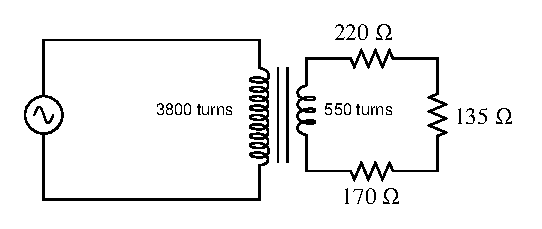
\includegraphics[width=15.5cm]{i01267x01.eps}$$

\begin{itemize}
\item{} $V_{primary}$ = 
\item{} $V_{secondary}$ = 
\item{} $I_{primary}$ = 
\item{} $I_{secondary}$ = 
\end{itemize}

\underbar{file i01267}
%(END_QUESTION)





%(BEGIN_ANSWER)

\begin{itemize}
\item{} $V_{primary}$ = 21.04 volt
\item{} $V_{secondary}$ = 3.045 volt
\item{} $I_{primary}$ = 839.5 mikroampere
\item{} $I_{secondary}$ = 5.8 milliampere
\end{itemize}

%(END_ANSWER)





%(BEGIN_NOTES)

De fleste transformatoroppgaver handler i bunn og grunn om forholdstall, men noen studenter synes forholdstall er vanskelige å håndtere. Spørsmål som dette egner seg godt til at studenter kommer opp til tavlen og viser hvordan de kom frem til resultatene.

%INDEX% Electronics review: transformer ratios

%(END_NOTES)

